












































































































































































































































































































































































































































































































































































































































































































































































































































































































































































































































































































































































































































































































































































































































































































































































































































































































































































































































































































































































































































































































































































































































































































































































































































































































































































































































































































































































































































































































































































































































































































































































































































































































































































































































































































































































































































































































































































































































































































































































































































































































































































































































































\section{Modeling Technology}\label{sec:overview}

In this section we will describe how we modeled and developed exhaustive embedding-based search on GPU with attribute-based matching. We will provide details on how we scaled our model-based index to billion size on a single GPU with quantization. We extend Mixture of Logits (MoL) \cite{MoL_paper} by automatically training cluster embedding components and experimenting with different gating functions and variety of embedding components.

\subsection{Exhaustive Search with Attribute-Based Matching (ABM)} \label{sec:knn}

Considering the post-filtering (filter after similarity-based retrieval) often suffers from the liquidity issue especially combining with ANN algorithms implemented on GPUs \cite{zhao2022constrained}, we first focus on the KNN-based algorithm with attribute-based pre-filtering and introduce several basic approaches adopted to tackle the above challenges.  Strategies to further improve the algorithm and tackle other online serving challenges including the live update problem will be introduced in \S\ref{sec:system_deployment}.

%{\color{red} Future exploration GPU-based implementation could be ... on ... [ref ping's work ANN filter].}
%{\color{red} QQ: we need a figure here for the two approaches}


\begin{figure}
    \centering
    \vspace{-4pt}
    \begin{adjustbox}{max size={\linewidth}{\textheight}}
        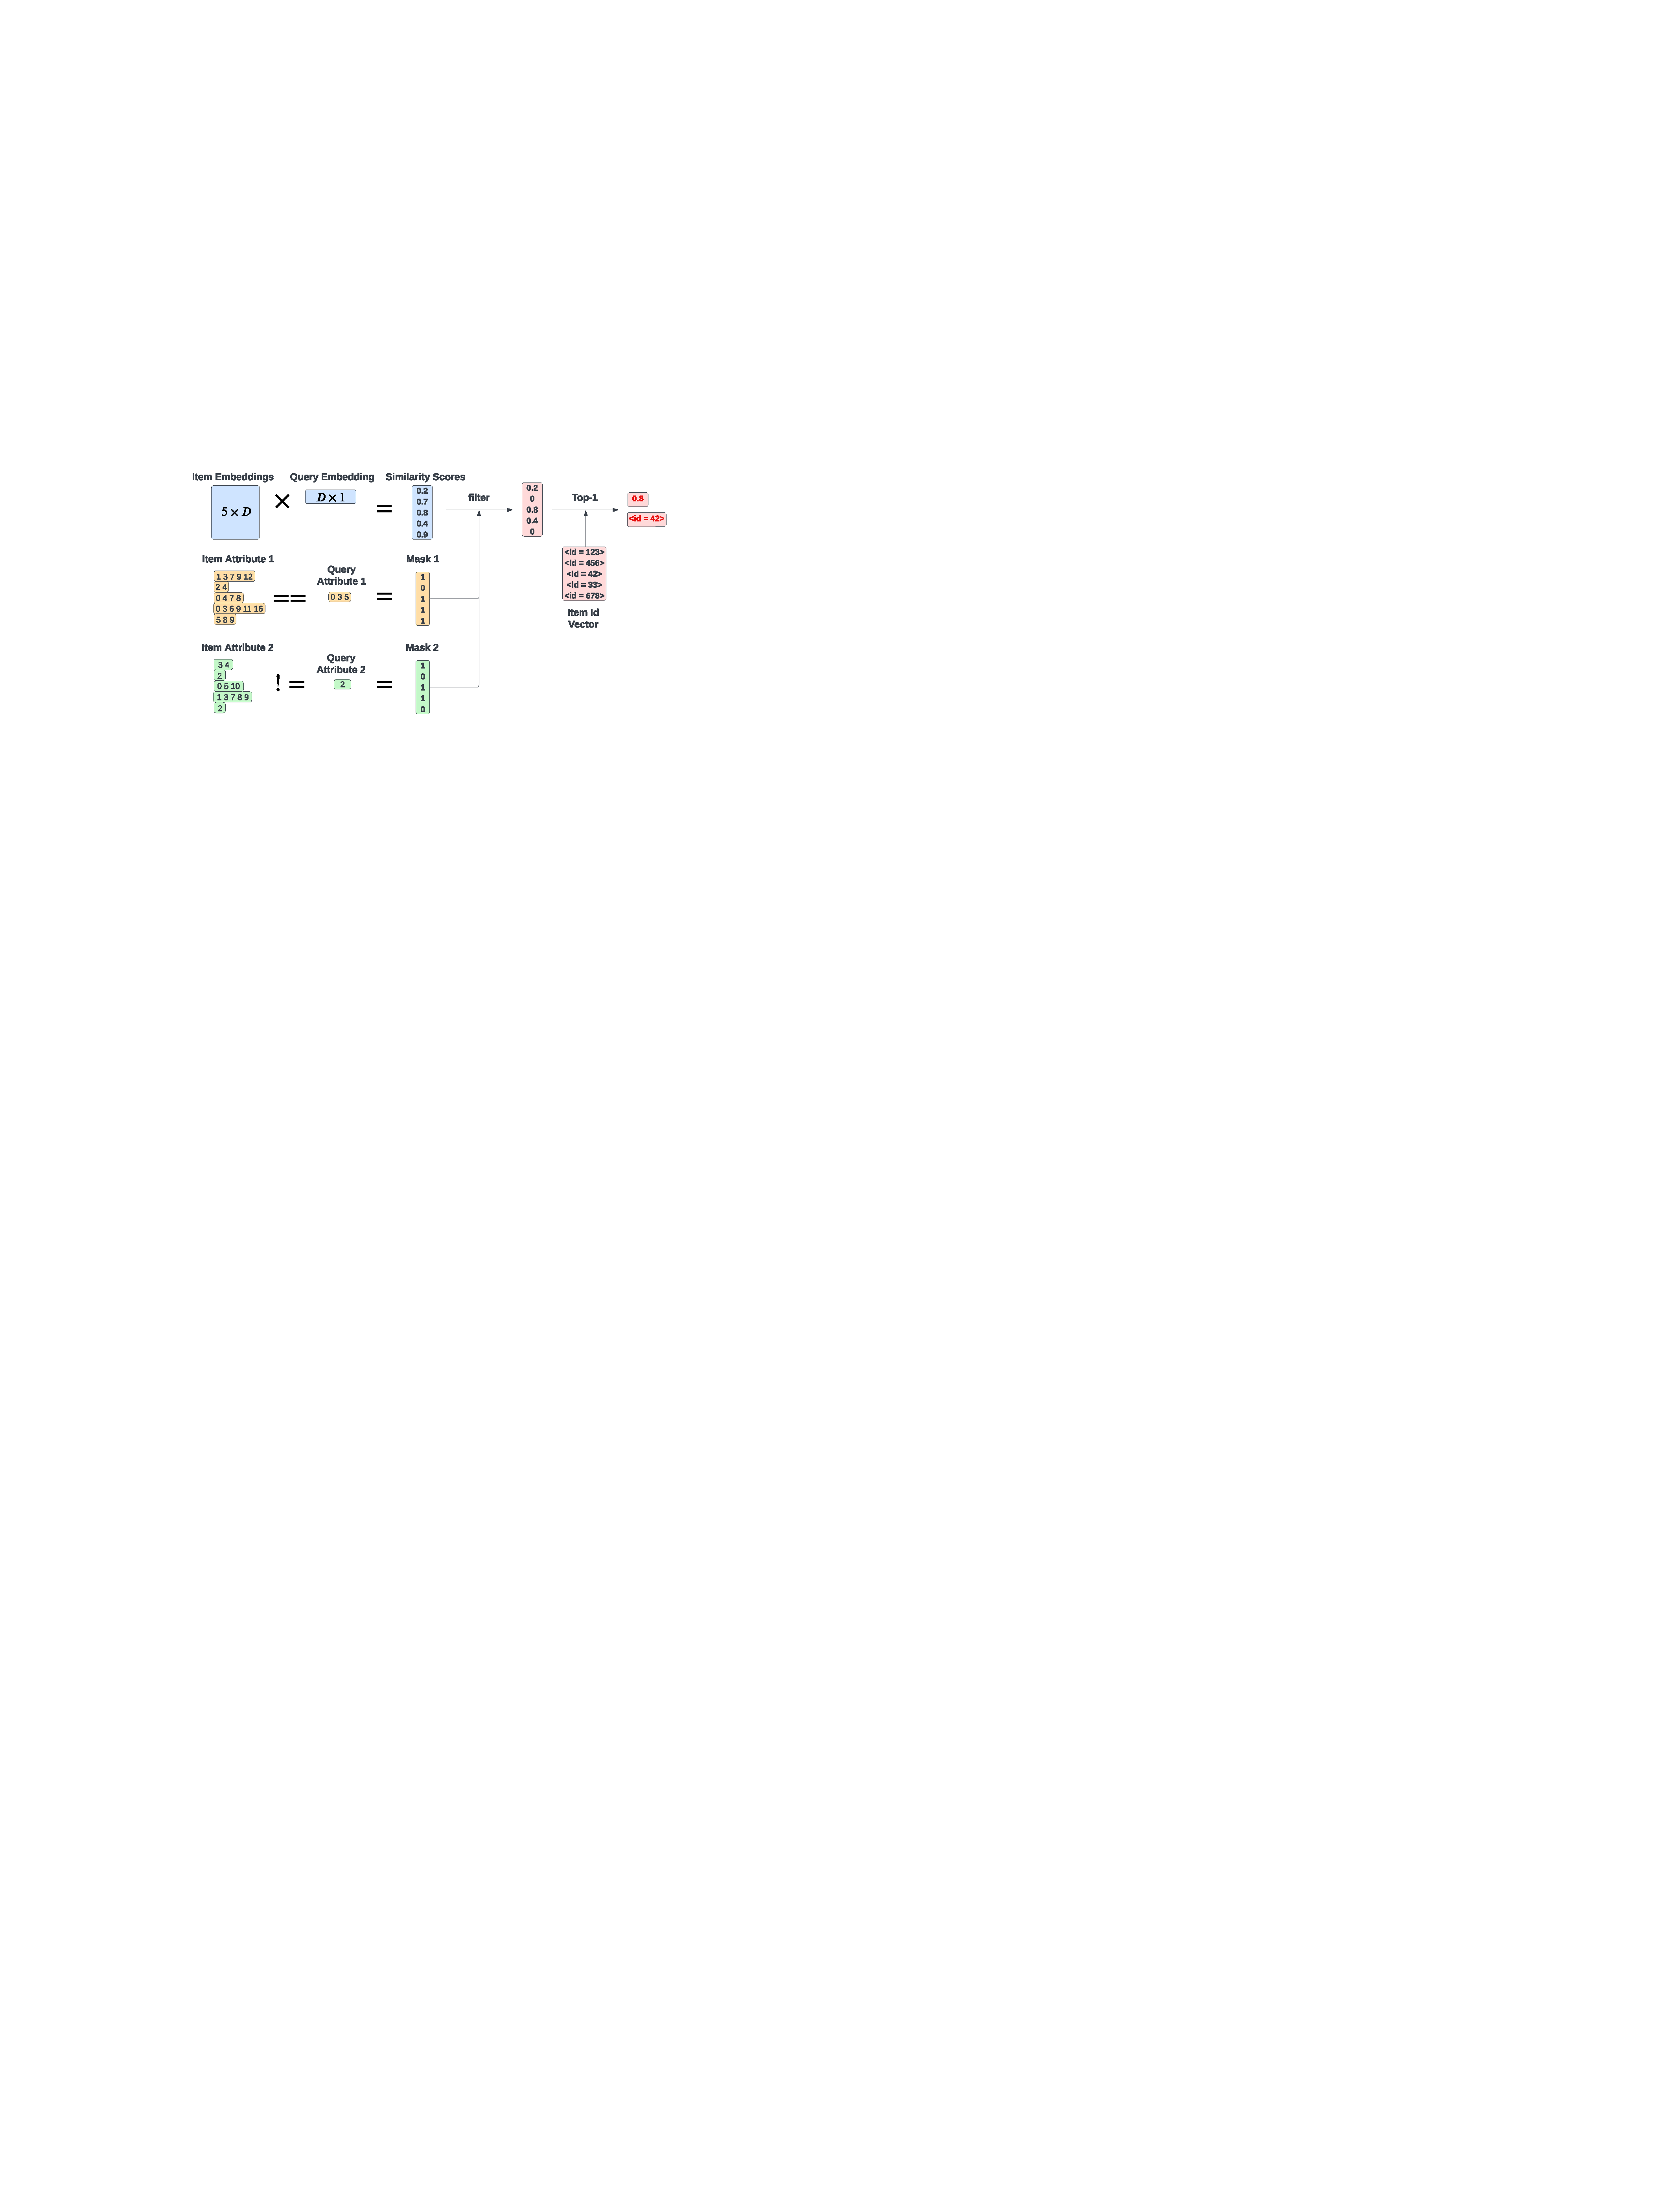
\includegraphics{figures/knn_v1.pdf}
    \end{adjustbox}
    \caption{
    \small
    %KNN with Similarity Masking: We illustrate with five items and a single query. Item similarities are computed and masked with two 0-1 vectors returned from two clause checking. If any item attribute matches the query attribute, the clause is passed (returns one) in the masking matrix. The second clause is a reverse matching clause. Top-1 selection is used in this example. D represents the dimension of the item embedding.
    KNN with Similarity Masking. An example of five items with single query is used for illustration. Item similarities are computed and masked with two 0-1 vectors returned from the two clause checking. For each item, as long as one attribute is matched with the query attribute, the clause checking is passed (return one) in the masking matrix. The 2nd clause is a reverse matching clause. Top-1 selection is used in this example. D is dimension of item embedding.
    }
    \label{fig:knn-v1}
    \vspace{-16pt}
\end{figure}


\subsubsection{KNN with Similarity Masking}
Our first KNN algorithm with ABM is a two-step similarity masking approach. As shown in Figure~\ref{fig:knn-v1}, given a query, we first compute the similarity between the query embedding with all item embeddings stored in a matrix to capture their semantic relationships in a similarity vector. Then, we filter out irrelevant items by multiplying it with the 0-1 mask vectors given by each clause to map the similarity scores of the filtered items to zero before the top-K selection. Each query clause could contain multiple attributes. Feasible items should satisfy all clauses, requiring at least one of the attribute in each clauses is matched. Reverse clauses are also supported (such as the company name attributes in Figure~\ref{fig:knn-v1}). As each item could contain different number of attributes for each clause, to effectively utilize the GPU memory for saving and update the clauses, we store all clause attributes in a single matrix in practice and have an extra counting matrix to record the number of attributes for each item in each clause similar to the counting matrix in a CSR format but for each item separately without having the indexing vector. Each item clause is sorted before the concatenation for faster judgement (as we can stop checking early as long as one attribute is matched). We implement the algorithm in CUDA and registered the clause filtering kernel as TensorFlow and PyTorch operations to integrate and serve with other modules.

% This version aims to strike a balance between computational efficiency and accuracy in identifying the nearest neighbors.

% This filtering step is crucial for optimizing the subsequent top-k selection process, ensuring that only the most relevant items are considered. 



\begin{figure}
    \centering
    \vspace{-4pt}
    \begin{adjustbox}{max size={\linewidth}{\textheight}}
        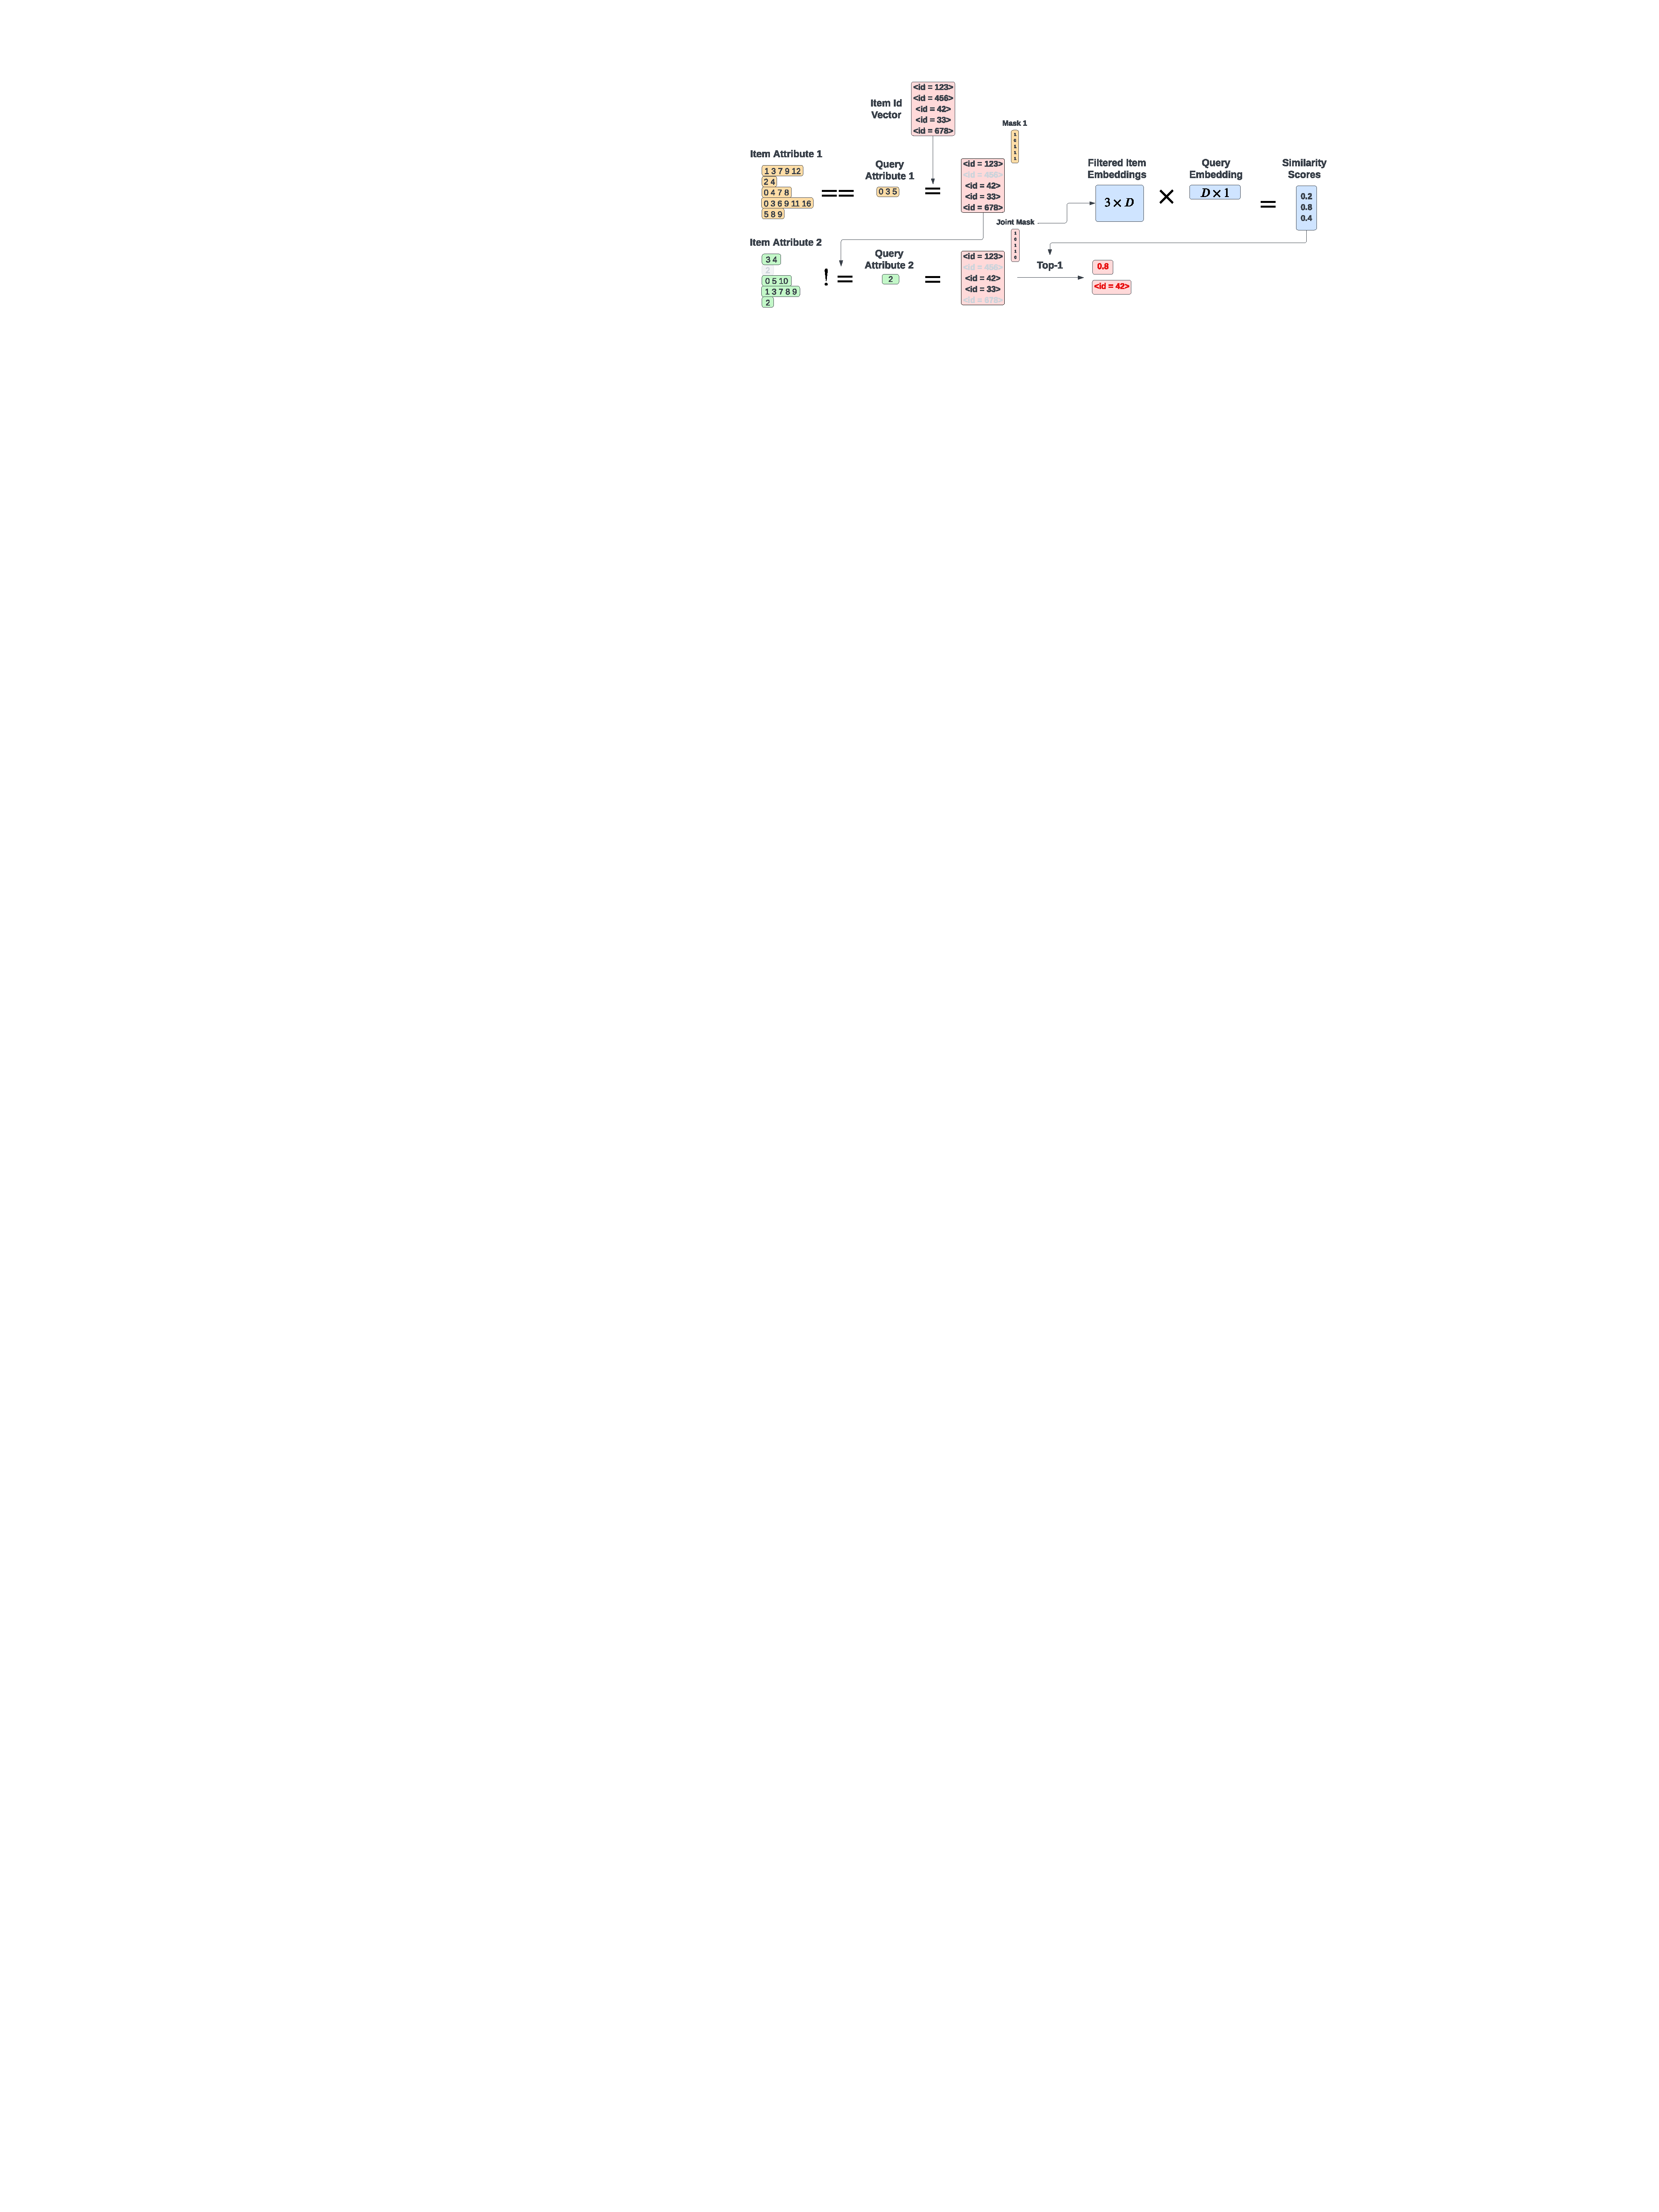
\includegraphics{figures/knn_v2.pdf}
    \end{adjustbox}
    \caption{\small KNN with Explicit Pre-Filtering. Clauses are checked one by one and a joint 0-1 mask vector is returned to retrieve the feasible items for matrix multiplication and top-K selection (K=1 here).}
    \label{fig:knn-v2}
    \vspace{-12pt}
\end{figure}

\subsubsection{KNN with Explicit Pre-Filtering}\label{sec:prefilter}
The second iteration of our KNN with ABM uses a new approach, incorporating explicit filtering before embedding multiplication, as illustrated in Figure~\ref{fig:knn-v2}. Initially, we slice the matrix to filter out irrelevant items, removing them early from subsequent computations. This method speeds up the process by reducing the computational burden during matrix multiplication and top-K selection, especially beneficial when the query filters result in a significantly smaller item set. We found that with custom CUDA implementation \cite{shen2024learningretrievejobmatching} to merge the kernels, the speed could be generally faster than the first version introduced above. However, without customizing the masked matrix multiplication and kernel merging, simply adopting the matrix slicing in TensorFlow and PyTorch will introduce extra matrix copy and creation overhead, causing it to be slower than the first version when the pass rate is high.
%The second version of our KNN with ABM introduces a different strategy by incorporating explicit filtering before the embedding multiplication. As shown in Figure~\ref{fig:knn-v2}, we begin by filtering out irrelevant items through matrix slicing, and directly remove them from consideration in the subsequent computations. As clause filtering operation is much faster than the rests, this version aims to enhance efficiency by explicitly excluding irrelevant items early in the computation, potentially reducing the computational load during matrix multiplication and top-K selection especially when the passing rate is low during given the query filters, i.e., the refined set of items after the filtering process is much fewer than the original item set. Practically, we found that with good custom CUDA implementation to merge the kernels, the speed could be generally faster than the first version introduced above. However, without customizing the masked matrix multiplication and kernel merging, simply adopting the matrix slicing in TensorFlow and PyTorch will introduce extra matrix copy and creation overhead, causing it to be slower than the first version when the pass rate is high.

% Following this, we perform matrix multiplication to obtain a refined set of similarity scores. 

%The top-k selection process is then applied to identify the most relevant items based on these refined scores. 




\subsection{Quantized KNN}\label{sec:quant_knn}

% \subsection{Index Quantization}
% \todo{QQ to write how to fit large indexes to 1 GPU core}

%{\color{red} QQ: we need another figure here}
%To tackle the memory issue, we introduce a quantized KNN approach leveraging the Sign One Permutation One Random Projection (Sign-OPORP) approach~\cite{li2023oporp} to compress and quantize emeddings into 1-bit values and approximate the dot-product via bitwise-matching operator. This approach provides a trade-off between the prediction accuracy and search speed similar to the regular ANN approach but is an exhaustive search method that can be directly combined with attribute-based pre-filtering method to avoid the liquidity issue.
Addressing memory constraints, we adopt a quantized KNN strategy using the Sign One Permutation One Random Projection (Sign-OPORP) method to compress embeddings to 1-bit and approximate dot-products via bitwise matching. This technique balances prediction accuracy and search speed, akin to typical ANN methods, but as an exhaustive search, it seamlessly integrates with attribute-based pre-filtering, circumventing liquidity issues.
%for fast approximate similarity computation as extra prefilters. 
OPORP is a variant of count-sketch method. It leverages single random projection with fixed-length binning scheme to efficiently project embedding to a low-dimensional embedding. Sign-OPORP takes the sign of the projected embedding to generate 1-bit embedding that could accurately approximate the cosine similarity of the original floating-point embedding~\cite{li2023oporp} via bit-wise matching, i.e., counting the number of matched bits of two quantized 1-bit embedding.

As the bit-wise matching operation is often much faster than regular matrix multiplication, we can replace the original embedding with quantized embedding and adopt the bit-wise matching operations in the above-mentioned KNN algorithm with pre-filtering, which can help greatly reduce the memory consumption. Compressing 1 billion fp16 embedding of dimension 64 to 1-bit embedding of the same dimension can reduce the memory by 16 times and help serve 1 billion items in single V100 GPU. We could adjust the size of the quantized embedding to balance the trade-off between the memory/speed and accuracy. Besides, if memory is not the concern, we could leverage the approximated similarity as an extra pre-filtering step reduce the computation of the full-precision matrix multiplication (see Figure~\ref{fig:knn-v3}), offering a unique perspective on exhaustive KNN with ABM. Note that, we call it exhaustive KNN to discriminate it from the regular ANN method with clustering such as HNSW and IVFPQ since our approach still computes all item similarity based on the quantized embeddings, which is easier to be combined with the pre-filtered ABM and live updates (see \S\ref{sec:live_update}).


%This main idea of OPORP is to involves shuffling and quantizing embeddings to 1-bit representations, which are then packed into integers (int32 or int64). Using bit match, we compute an approximated similarity measure of cosine similarity more efficiently. 

%Similar to Version 1, a filtering step is employed, masking the similarity scores to zero for irrelevant items. After selecting the top-T items, matrix multiplication is performed on this refined set, and the final top-K items are selected. The OPORP quantization introduces a trade-off between quantization accuracy and computational efficiency, offering a unique perspective on KNN with ABM.

%{\color{red} Speed is also faster, so if memory issue is not a concern, we can put quantization as an extra filtering step after the clause filtering to further reduce the complexity of computing dot products.}


\begin{figure}
    \centering
    \vspace{-4pt}
    \begin{adjustbox}{max size={\linewidth}{\textheight}}
        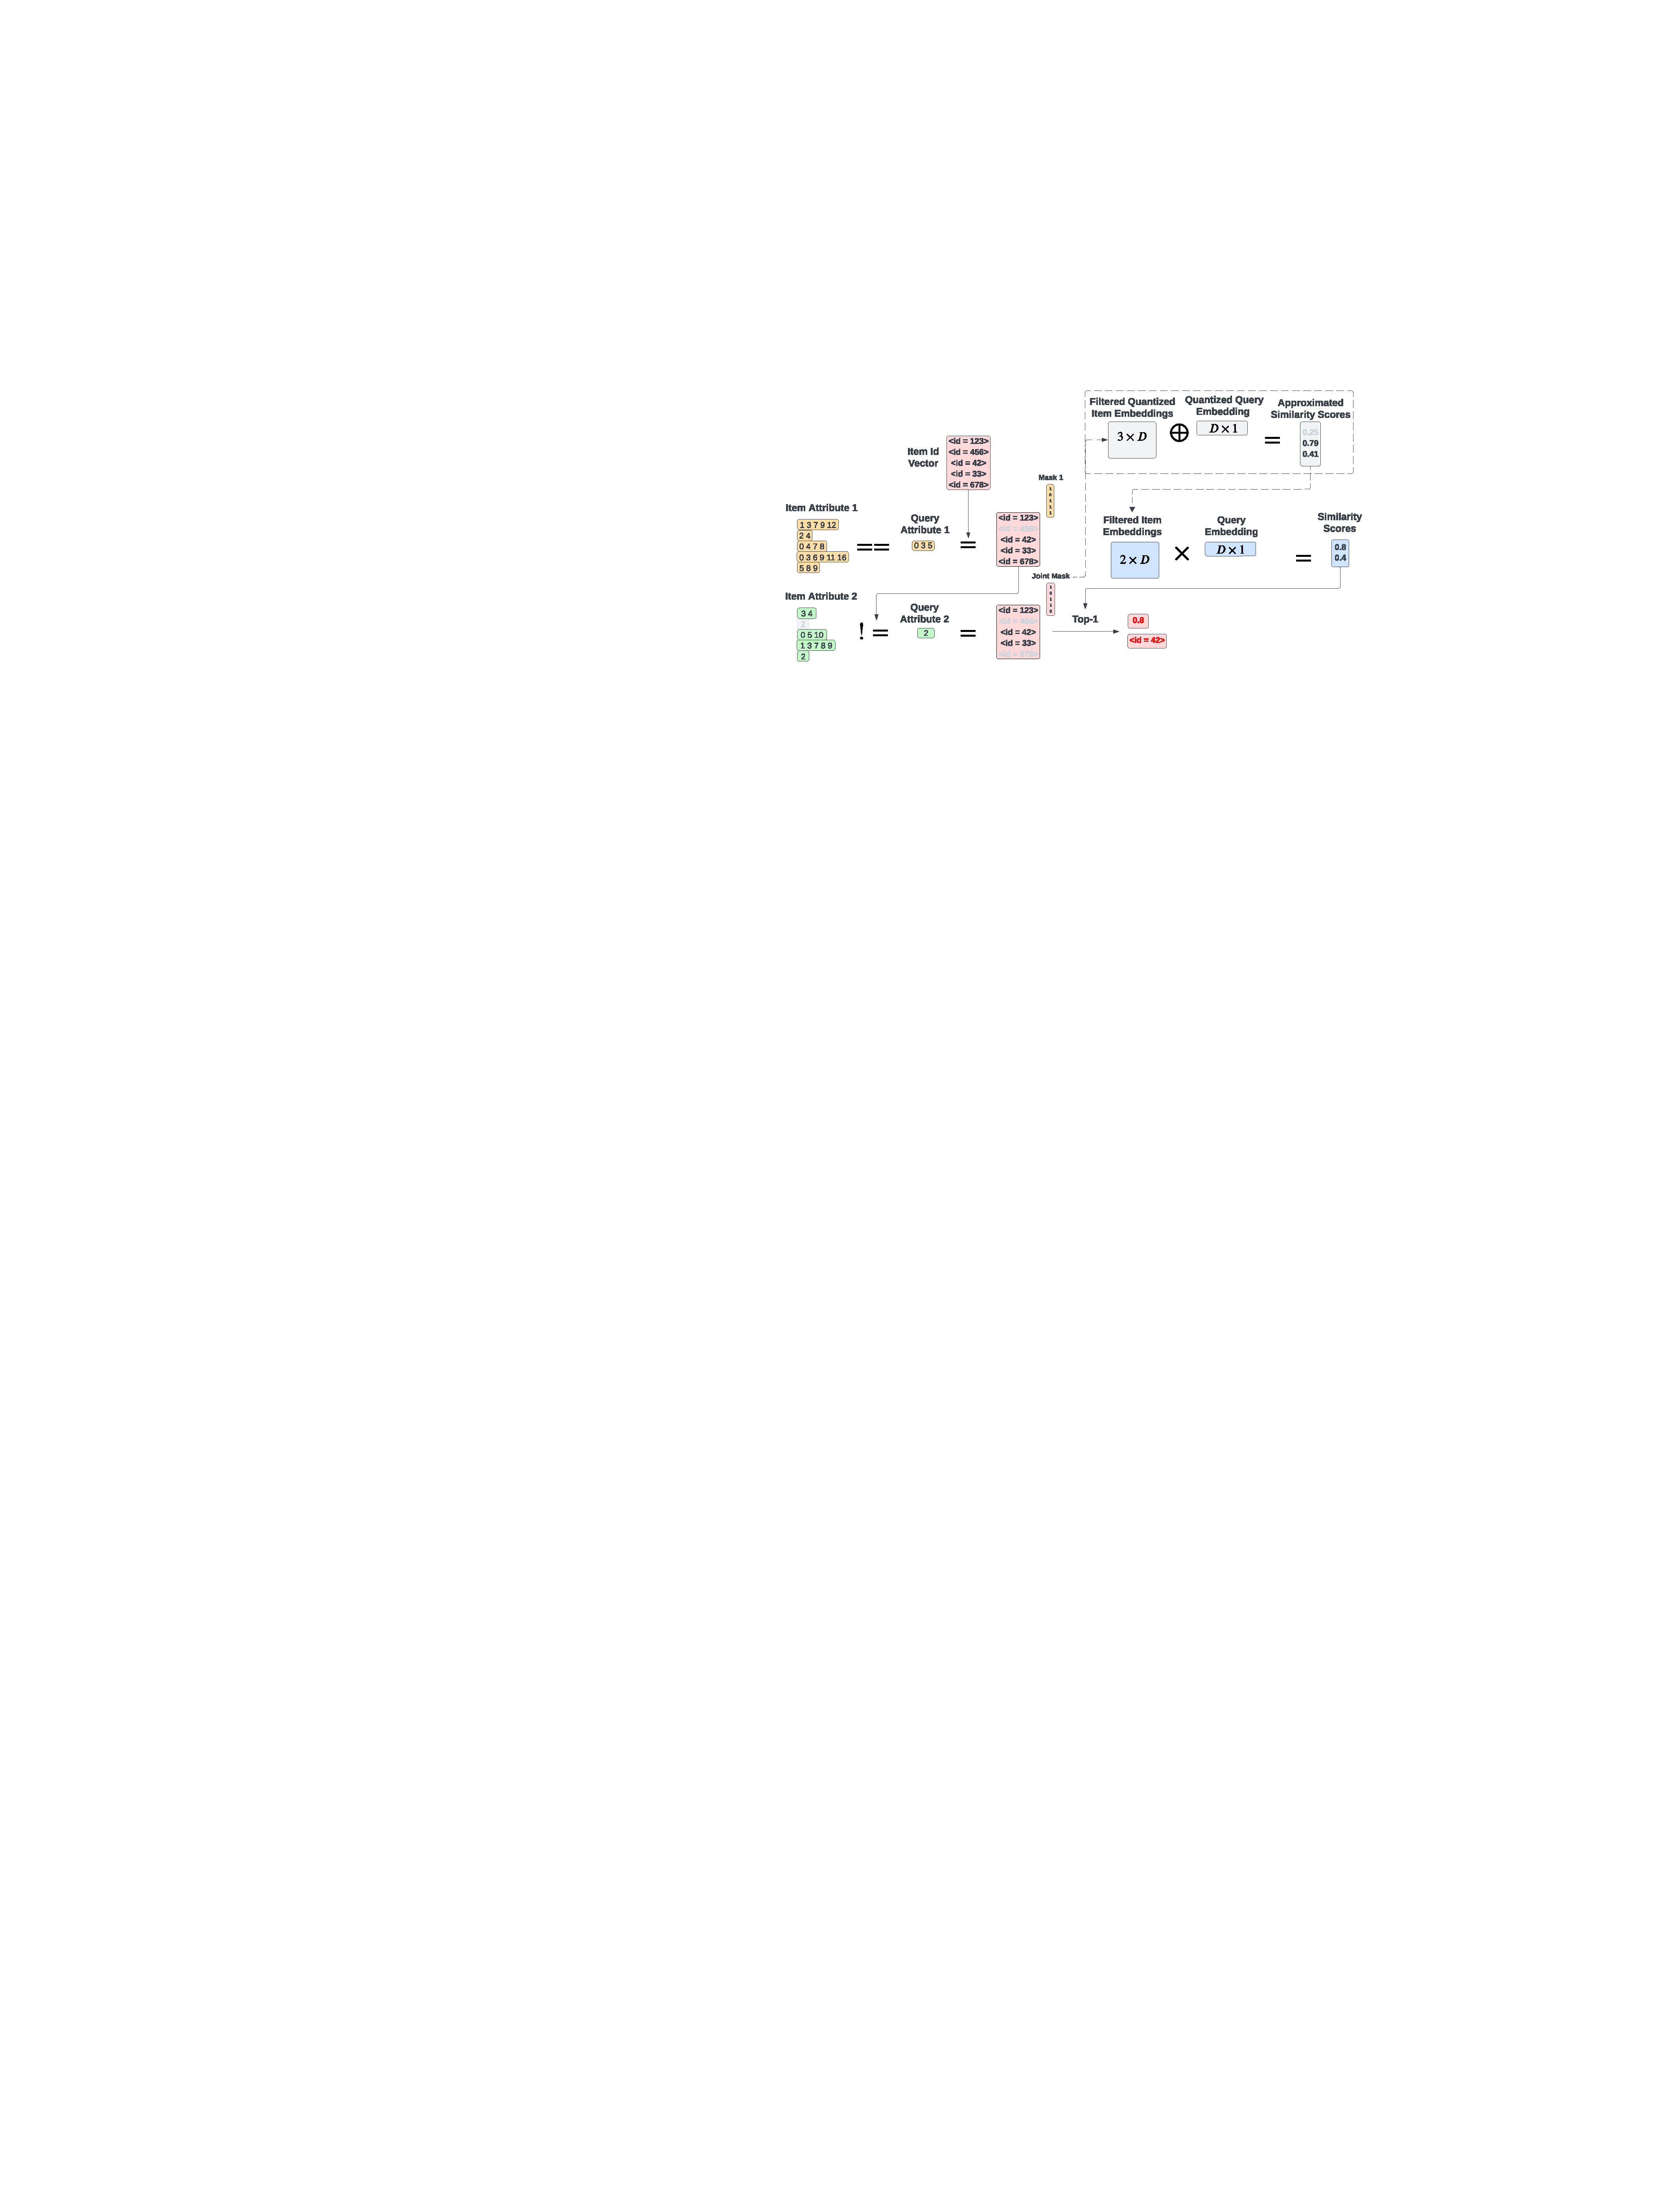
\includegraphics{figures/knn_v3.pdf}
    \end{adjustbox}
    \caption{\small KNN with Quantized Filtering helps to reduce the number of retrieved items before the full precision similarity computation. A bit-wise matching is used to measure the approximated similarity between 1-bit quantized embedding obtained via Sign-OPORP method. We use bit-wise XOR operation and perform an integer bit-wise NOT conversion for query or item embedding in advance to measure the number of matched bits in the packed integer vector. The quantized KNN module can be used without full precision matrix multiplication when K is large in top-K selection.}
    %The quantized KNN module could also be independently used without having to have the full precision matrix multiplication afterwards when the K value is large in the top-K selection.
    \label{fig:knn-v3}
    \vspace{-12pt}
\end{figure}

%% mizhou: change subsection title and add Hadamard MLP
% \subsection{Learnt clustering for Mixture-of-Logits}\label{sec:mexture_similarities}
\subsection{Similarity Modeling}\label{sec:mexture_similarities}

\subsubsection{Hadamard MLP}
Dot Product or cosine similarity has been common in retrieval and it’s computationally efficient. On the other hand, the multilayer perceptron (MLP)-based learned similarity functions has been reported inferior compared to properly tuned dot product. To balance the computation cost/latency and retrieval metrics, we attempted to boost the MLP-based learned similarity function through hadamard product. The architecture is shown on the left of Figure \ref{fig:Residual_learning}. A MLP block is applied to member and item embedding respectively, whose output performs hadamard product and then passes to another MLP block to output the final logit. With proper hyper-parameter tuning, it can reliably outperform dot product.

\subsubsection{Mixture-of-Logits with Clustering}
Mixture-of-logits ~\cite{MoL_paper} defines a model for computing high rank similarity based on adaptive gating of elementary logits across multiple embedding components $\phi_{MoL}(x, u) = \sum\limits_k \pi_{k,\theta}(x, u) \delta_{k,\theta}(x, u)$, where $\pi_{k,\theta}(x, u)$ represents a learnt gating function, which gives per component weight using soft-max gate given input of user and item features. The parameters $\theta$ are learnt through Adam optimization of gradients of a sampled soft-max loss. 
%\begin{equation}
%\small
%$\phi_{MoL}(x, u) = \sum\limits_k \pi_{k,\theta}(x, u) \delta_{k,\theta}(x, u)$
%\end{equation}

\begin{comment}
The authors of MoL used dot product as their similarity function in production settings:
\begin{equation}
\Phi_{\text{MoL dot products}}(x, u) = \sum_k \pi_{k,\theta}(x, u) <f_{k,\theta}(u), g_{k,\theta}(x)> 
\label{eq:MoL} 
\end{equation}
\end{comment}

% $f_{k,\theta}()$ and $g_{k,\theta}()$ are different learnable functions for the raw user and item embeddings. 

\begin{comment}
MoL paper lacks specificity how different MoL components $f_{k,\theta}(u)$ and $g_{k,\theta}(x)$ are trained. To fill the gap we provide variety of methods to generate $f_{k,\theta}()$ and $g_{k,\theta}()$ embedding components for MoL in subsections \S\ref{sec:residual_IDs} and \S\ref{sec:offline_evaluation}.
\end{comment}

\begin{comment}
\cite{MoL_paper} mentions that dot product similarities can outperform multilayer perceptron (MLP)-based learned similarity functions. In contrast we extend the formulation to provide set of learnt distances $F_{i}$ with MLP layers including weighted inner product \cite{weighted_dot_product} represented by a single linear layer and Hadamard MLP learnt with few fully connected layers \cite{wang2022flashlight}:
\begin{equation}
\Phi(x, u) = \sum_{F_{i} \in \text{ MLP similarities}} \sum_k \pi_{k,\theta}(x, u) F_{i}(f_{k,\theta} (u), g_{k,\theta}(x))
\label{eq:mixture_of_similarities}
\end{equation}
\end{comment}

Mixture-of-logits requires the availability of multiple features to leverage the gates, because the gates will collapse to a value of 1 if there is only one feature for user and item pair. We augment the feature with learnt cluster id embedding that obviate the necessity for having multiple features.
In \S\ref{sec:offline_evaluation} we show that learnt cluster id embedding leveraged through Mixture-of-Logits
can significantly improve on top of dot product in production settings.

% \subsubsection{Learning cluster id embedding for Mixture-of-Logits}\label{sec:residual_IDs}
Across LinkedIn we observed variety of member behaviour with some members coming frequently and some coming from time to time. For the infrequent members we aimed to improve retrieval system performance. To achieve this we learn cluster id embeddings, which represent interests of cohorts of members and topics of posts. We describe the process on the right of Figure \ref{fig:Residual_learning}. 

% Given two tower embeddings of members and posts, we cluster them using Kmeans++ in offline and store cluster centers as part of the {\systemname} model.

For training {\systemname}, we obtain two-tower embeddings for posts and members as part of the training data, along with available engagement labels. We initialize cluster ID embeddings using K-means on millions of post embeddings. During training for both members and posts, we find the closest cluster ID embedding based on cosine similarity to their two-tower embedding. These cluster IDs for members and posts are integrated into Mixture-of-Logits, along with the original two-tower embedding and other embeddings we developed for our use cases. We experimented with using K-means-initialized cluster ID embeddings as is and fine-tuning them through back propagation. We report the experiment results in \S\ref{sec:offline_evaluation}.

\begin{comment}
During training and inference given the member or post embeddings we infer cluster centers associated with it by dot product of post or member two tower embedding with cluster centers. We take top $K$ clusters. For each of the cluster IDs we train respective clusterID embeddings as part of the model based on the member's engagement data, which means that clusters represent engagement patterns of those topics. ClusterID's usage in the model as a sparse ID feature is a common technique \cite{visrel_paper}. In this paper we propose to extend clusterID features and train them jointly with personalized ID embeddings for popular members and posts and sum them together in the model for more robust feature representation. Combination of clusterID with personalized IDs helps to improve learning for cold start items/members and kicks in personalization given even few engagement points for items/members via personalized ID embeddings. Cluster IDs can be seen as initialization for personalized ID embeddings due to sum combination in the model. Member ID and post ID embeddings are randomly initialized closely to zero. ClusterID embeddings could be initialized randomly or with offline kmeans centroid values. We found that performance is the same with longer training for both initialization methods.
\end{comment}

\begin{figure}
    \centering
    \vspace{-4pt}
    \begin{adjustbox}{max size={\linewidth}{\textheight}}
        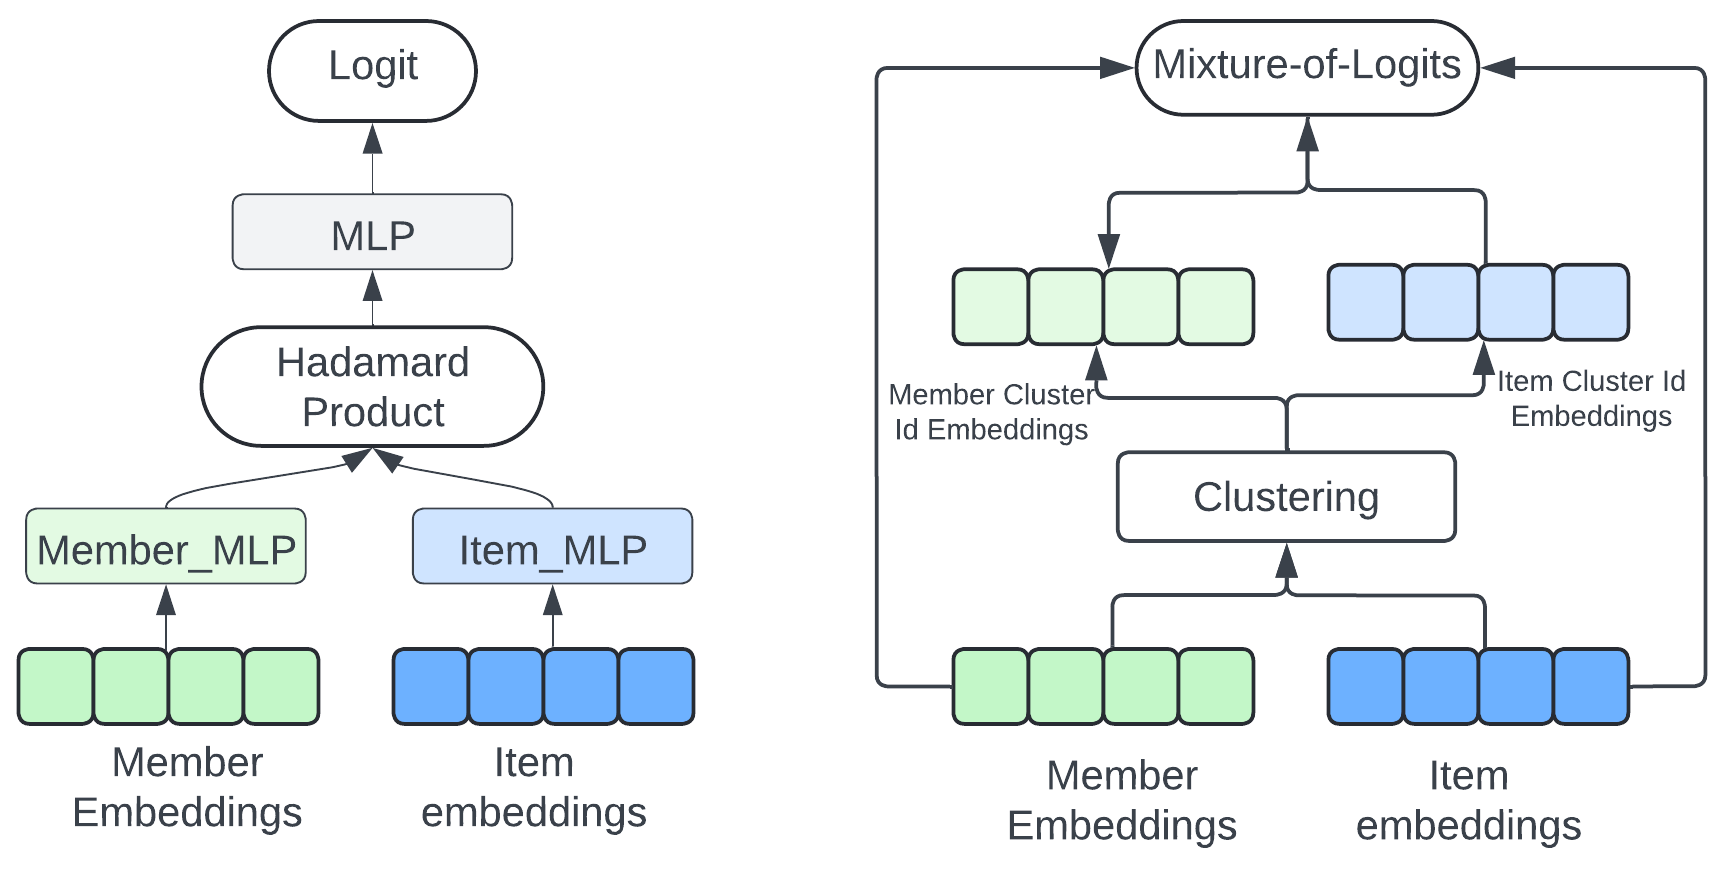
\includegraphics[scale=0.1]{figures/similarity_modeling.png}
    \end{adjustbox}
    \caption{\small Illustration of Hadamard MLP (left) and learning cluster id embedding for Mixture-of-Logits(right)}
    \label{fig:Residual_learning}
    \vspace{-12pt}
\end{figure}
